\documentclass{amsart} 
\usepackage{amsfonts}

%     If your article includes graphics, uncomment this command.
\usepackage{graphicx} % Required for including images
%\graphicspath{{../Figures/}} % Set the default folder for images

\usepackage{prettyref}
\usepackage[utf8]{inputenc}
\usepackage{bm}


%\numberwithin{equation}{section}

%    Absolute value notation
\newcommand{\abs}[1]{\lvert#1\rvert}

%    Blank box placeholder for figures (to avoid requiring any
%    particular graphics capabilities for printing this document).
\newcommand{\blankbox}[2]{%
	\parbox{\columnwidth}{\centering
		%    Set fboxsep to 0 so that the actual size of the box will match the
		%    given measurements more closely.
		\setlength{\fboxsep}{0pt}%
		\fbox{\raisebox{0pt}[#2]{\hspace{#1}}}%
	}%
}

\begin{document}
	
	\title{\textit{Live Orchestral Piano}, a system for real-time orchestral music generation}
	
	%    Information for first author
	\author{Léopold Crestel}
	%    Address of record for the research reported here
	\address{Représentations musicales, \textit{IRCAM}, Paris, France 750104}
	%    Current address
	\email{leopold.crestel@ircam.fr}
	
	%    Information for second author
	\author{Philippe Esling}
	\address{Représentations musicales, \textit{IRCAM}, Paris, France 750104}
	\email{philippe.esling@ircam.fr}
	
	%    General info
	%	\subjclass[2000]{Primary 54C40, 14E20; Secondary 46E25, 20C20}
	
	\date{\today}
	
	%	\dedicatory{This paper is dedicated to our advisors.}
	
	\keywords{Automatic orchestration, Conditional Restricted Boltzmann Machine, Deep learning}
	
	\begin{abstract}
	This paper introduces the first system for performing automatic \textit{orchestration} based on a real-time piano input. We believe that it is possible to learn the underlying regularities existing between piano scores and their orchestrations by notorious composers, in order to automatically perform this task on novel piano inputs. To that end, we investigate a class of statistical inference models called \textit{conditional Restricted Boltzmann Machine} (\textit{cRBM}). We introduce a specific evaluation framework for orchestral generation based on a prediction task in order to assess the quality of different models. As prediction and creation are two widely different endeavours, we discuss the potential biases in evaluating temporal generative models through prediction tasks and their impact on a creative system. Finally, we introduce an implementation of the proposed model called \textit{Live Orchestral Piano} (LOP), which allows to perform real-time projective orchestration of a MIDI keyboard input.
	\end{abstract}
	
	\maketitle
	\section{Introduction}
	% Orchestration classique
	%% Musical orchestration : why is it so hard ?
	% Orchestration
	\textit{Orchestration} is the subtle art of writing musical pieces for the orchestra, by combining the properties of various instruments in order to achieve a particular sonic rendering \cite{koechli_orch,Rimsky-Korsakov:1873aa}. Because it extensively relies on spectral characteristics, orchestration is often referred to as the art of manipulating instrumental timbres \cite{mcadams2013timbre}. Timbre is defined as the property which allows listeners to distinguish two sounds produced at the same pitch and intensity.
	% -> Timbre
	Hence, the sonic palette offered by the pitch range and intensities of each instrument is augmented by the wide range of expressive timbres produced through the use of the different playing styles.
	%Hence, above the traditional harmonic and rhythmic structures, timbre becomes a crucial structuring dimension in orchestral works. 
	% Non linear spectral behaviours
	Furthermore, it has been shown that some instrumental mixtures can not be characterized by a simple summation of their spectral components, but can lead to a unique \textit{emerging timbre}, with phenomenon such as orchestral blend \cite{tardieu2012perception}.
	% -> Combinatoire
	Given the number of different instruments in a symphonic orchestra, their respective range of expressiveness (timbre, pitch and intensity), and the phenomenon of emerging timbre, one can foresee the extensive combinatorial complexity embedded in the process of orchestral composition.
	
	Those difficulties have been a major obstacle towards the construction of a scientific basis for the study of orchestration. From a mathematical point of view, it seems that no set of descriptors can exhaustively fit with the perceptual complexity of timbre \cite{peeters2011timbre}. From a musical point of view, there is a lack of specific symbolic notation for timbre, and orchestration remains an empirical discipline taught through the observation of existing orchestration examples \cite{piston-orch}. Among the different writing techniques for orchestral works, one of them consists in first writing an harmonic and rhythmic structure in the form of a piano score and then adding the timbre dimension by spreading the different voices over the various instruments \cite{piston-orch}. We refer to this operation of extending a piano draft to an orchestral score as \textit{projective orchestration} \cite{eslingthesis}.
	
	\begin{figure}
		\centering
		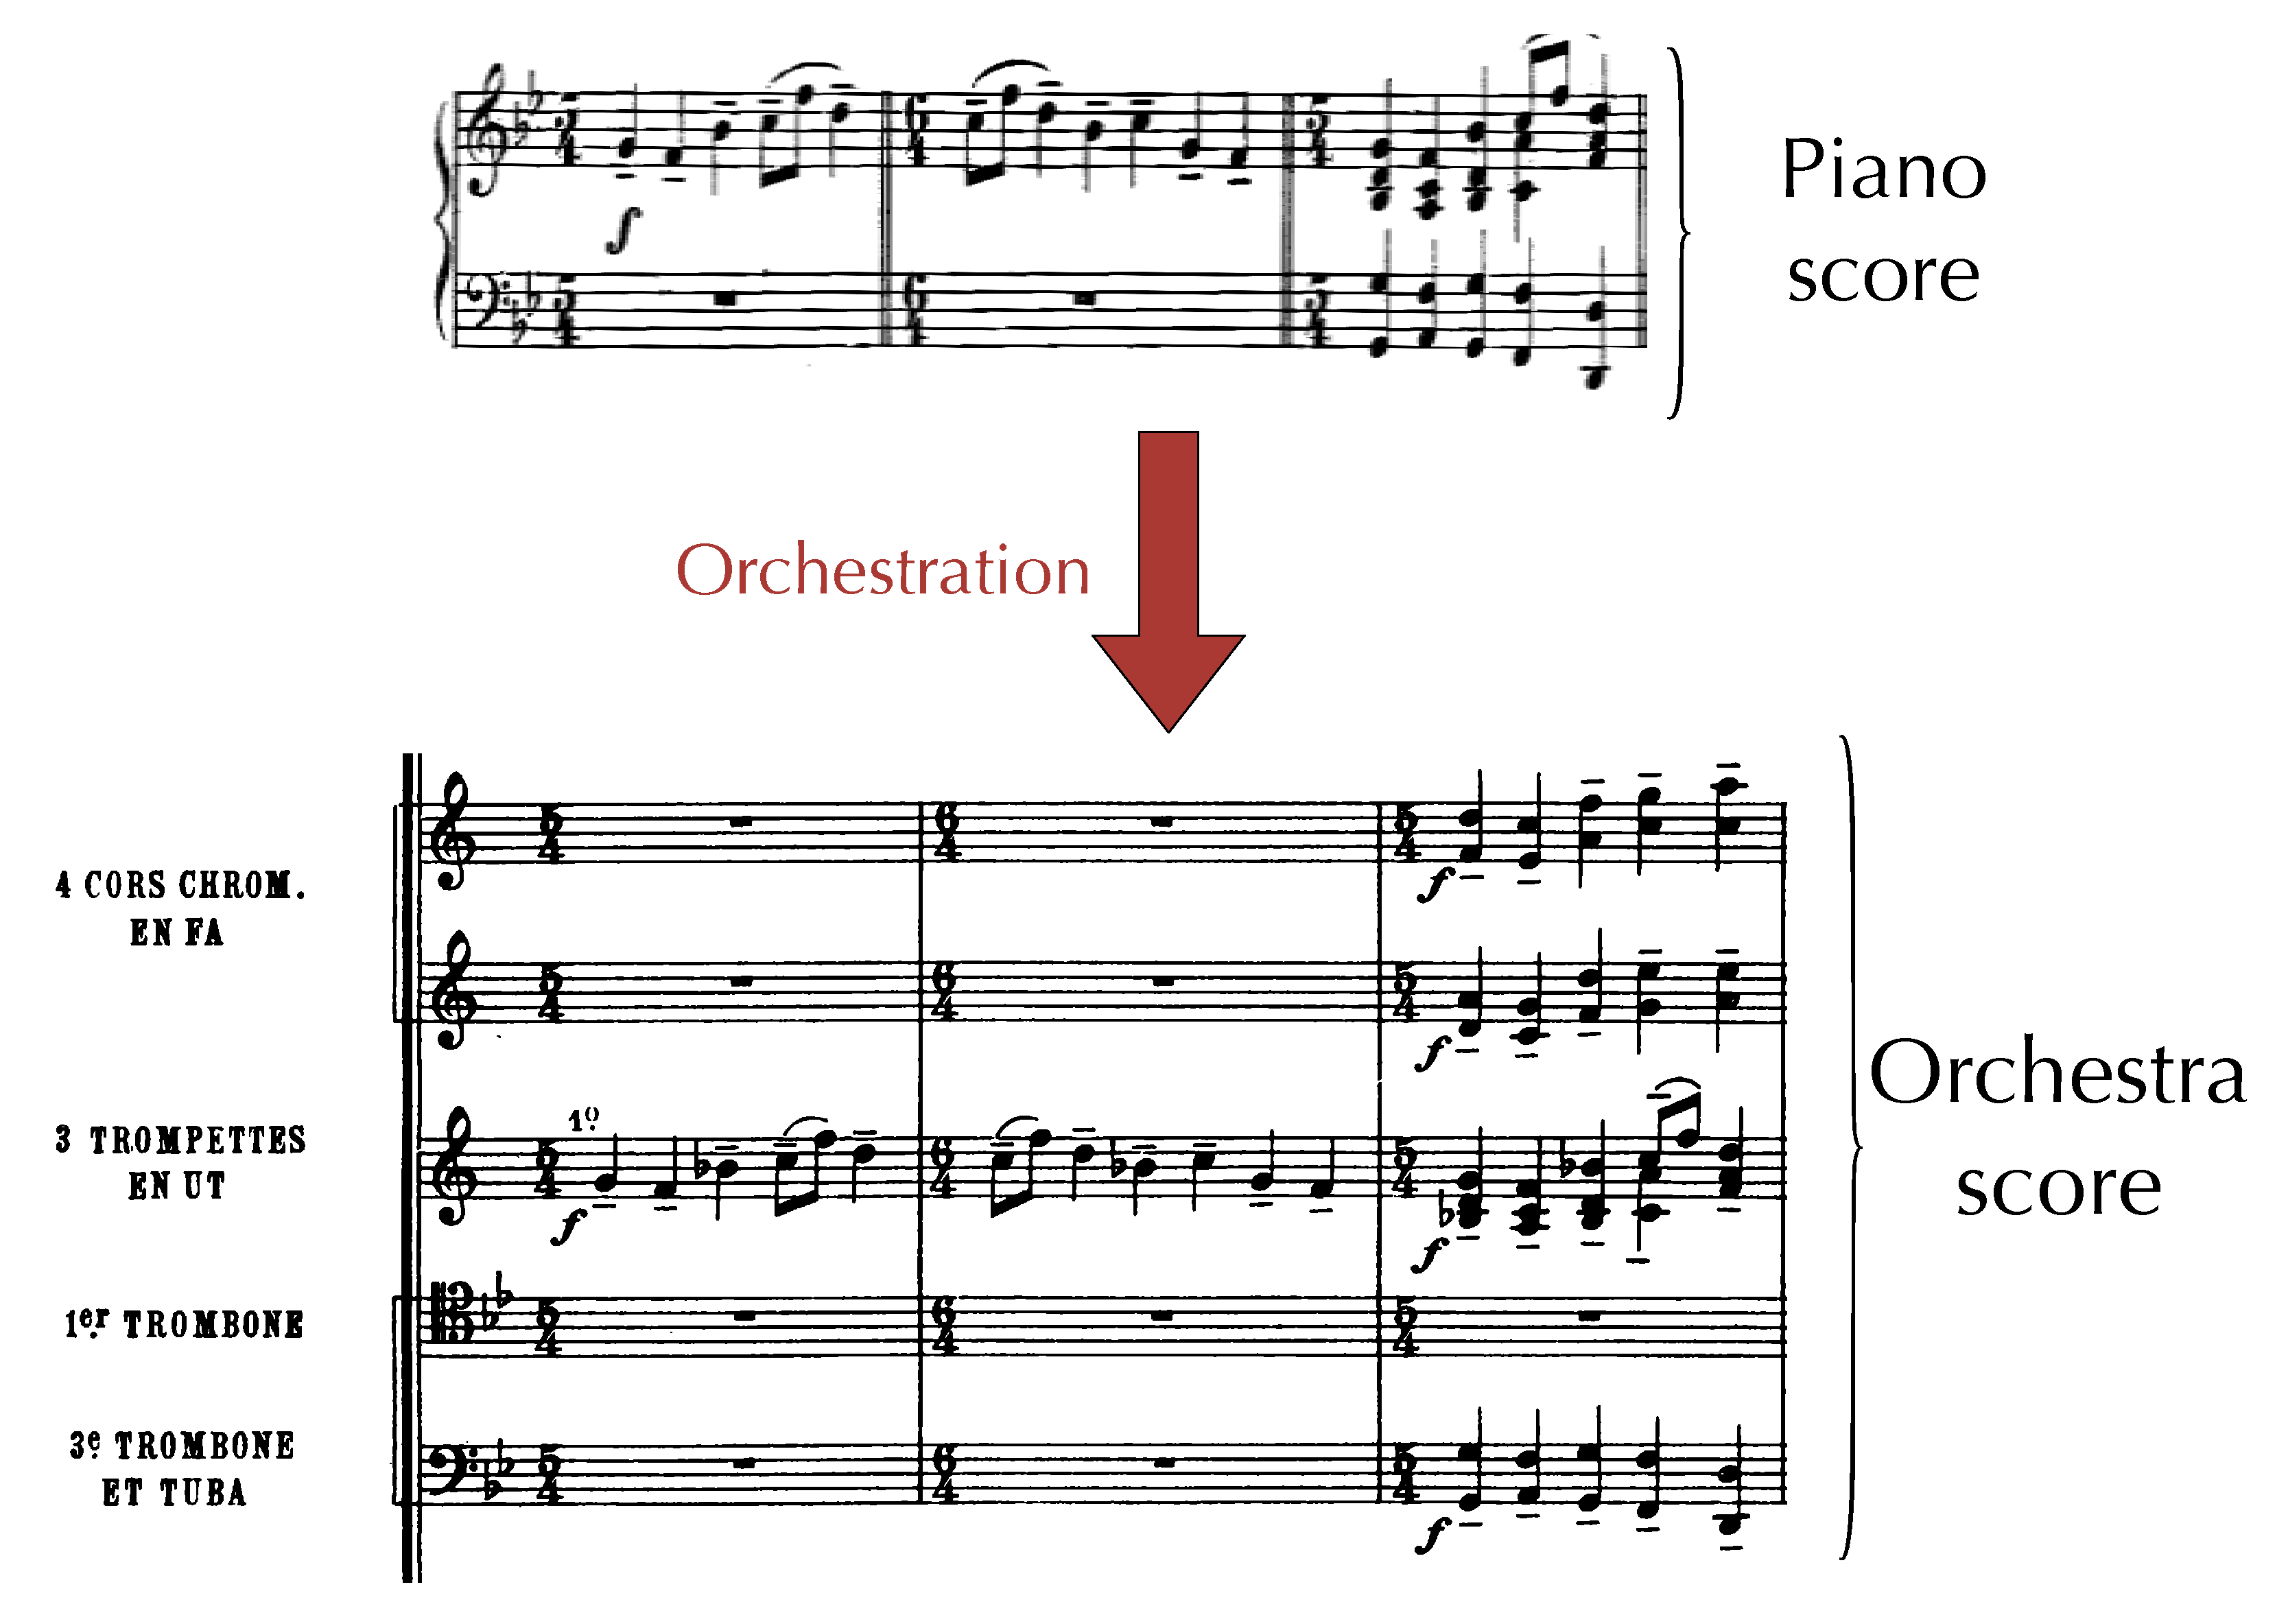
\includegraphics[scale=0.12]{orch.pdf}
		\caption{\textit{Projective orchestration}. A piano score is projected on an orchestra. Even though a wide range of orchestrations exist for a given piano score, all of them will share strong relations with the original piano score. One given orchestration implicitly embeds the knowledge of the composer about timbre and orchestration.}
		\label{fig:orch}
	\end{figure}
	
	The orchestral repertoire contains a large number of examples of projective orchestration (such as the piano reductions by Liszt of Beethoven symphonies or the \textit{pictures at an exhibition}, a piano piece by Moussorgsky orchestrated by several notorious composers). By observing a case of projective orchestration (see \prettyref{fig:orch}), we can clearly see that this process involves more than the mere allocation of notes written on the piano score across the different instruments. It rather implies harmonic enhancements and timbre manipulations to underline the already existing harmonic and rhythmic structure \cite{mcadams2013timbre}. However, the visible correlations between a piano score and its orchestrations appear as a fertile framework for laying the foundations of a computational exploration of orchestration. Even though systemic rules remain difficult to identify because of the high dimensionality of the problem, preventing us from building a general theory of orchestration, it does not mean that underlying local regularities could not be extracted.
	
	Statistical inference covers a range of methods aimed at automatically extracting a structure from observations. These approaches hypothesize that a particular type of data might be structured by an underlying probability distribution. The objective is to deduce properties of this distribution, by observing a set of those data. 
	If the structure of the data is efficiently extracted and organized, it should be possible in turn to generate novel examples.
	%Thus, our objective is to build a system of automatic projective orchestration. 
	We believe that learning the underlying distribution of a corpus of piano scores and their orchestrations by famous composers through statistical inference is a promising lead toward the automatic generation of orchestrations with a sensible timbre structure.
	In the context of projective orchestration, the data are defined as the scores, formed by a series of pitches and intensities for each instrument. The set of observations is the set of projective orchestrations performed by famous composers, and the probability distribution would model the set of notes played by each instrument conditionally on the corresponding piano score.
	
	It might be surprising at first to rely solely on symbolic information (scores) whereas we insisted on the fact that orchestration is the art of timbre, typically not represented in the musical notation but rather conveyed in the signal information (audio recording).
	However, we make the assumption that spectrally consistent orchestrations could be generated from a purely symbolic learning by uncovering the composers' knowledge about timbre embedded in the score. As we rely on the works of composers that effectively took into account the subtleties of timbral effects, these symbolic relationships embed the spectral information.
	
	A wide range of statistical inference models have been devised, among which deep learning recently appeared as a  promising field in artificial intelligence and representation learning \cite{bengio2013representation,LeCun:2015aa}. The building blocks of many models in this field is the \textit{Restricted Boltzmann Machine} (\textit{RBM}) \cite{hinton2006fast}.
	We focus on a class of models called \textit{Conditional RBM} \cite{taylor2006modeling}, which implements a notion of context particularly adapted to represent both the temporal dependencies in the orchestral score and the influence of the piano score.
	Besides these structural advantages, those models are also generative, which means that once the underlying distribution of the observed data is correctly modelled, it is possible to generate orchestration from unseen piano scores.
	
	In order to rank the different models, it is important to devise a quantitative evaluation framework. Designing a criterion assessing the performance of a generative model is a major difficulty for creative systems. In the polyphonic music generation field, a predictive task is commonly used \cite{DBLP:journals/corr/YaoCVDD15,boulanger2012modeling,lavrenko2003polyphonic}. Relying on these works, we introduce a specific framework for projective orchestration and discuss the results of the \textit{cRBM} and \textit{FGcRBM} models.
	
	Finally, an interesting property of both the \textit{cRBM} and \textit{FGcRBM} models is their ability to generate orchestration from an unseen piano score sufficiently fast for a real-time implementation.
	Using the defined performance criterion we selected the most efficient model and implemented it in a system called \textit{Live Orchestral Piano} (LOP), an interface for real-time orchestration from a piano input.
	
	The remainder of this paper is organized as follows. The first section introduces the state of the art in conditional models, in which RBM, cRBM and \textit{FGcRBM} models are detailed. The projective orchestration task is presented in the next section along with an evaluation framework based on a frame-level accuracy measure. The introduced models are evaluated within this framework and compared to existing models. Then, we introduce \textit{LOP}, the real-time projective orchestration system. Finaly, we provide our conclusions and directions of future work.
	
	\section{State of the art}
	In this section, three statistical inference models are detailed. The \textit{RBM}, \textit{cRBM} and \textit{FGcRBM} are presented by increasing level of complexity.
	
	\subsection{Restricted-Boltzmann Machine}
	The \textit{RBM} \cite{hinton2006fast} is a graphical probabilistic model (\prettyref{fig:RBM}) composed by a set of $I$ visible units $\bm{v} = (v_{1},...,v_{I})$, each representing a binary random variable. Those visible units usually model the observed data, in which case $I$ is equal to the dimension of the observed vectors. Note that this model can easily be extended to continuous variables \cite{hinton2010practical}. A set of $J$ binary random variables ($\bm{h} = (h_{1},...,h_{J})$) are called hidden (or latent) units. Hidden variables are not directly observed and model explanatory factors for the visible units distribution. They are connected to visible units through weights $W_{ij}$ which model conditional dependencies between the visible and hidden units activation
	\begin{align}
	\label{eq:marginal_RBM_1}
	p(h_{j}=1|\bm{v}) &= \sigma \left( b_{j} + \sum_{i}W_{ij}v_{i} \right)
	\end{align}
	\begin{align}
	\label{eq:marginal_RBM_2}
	p(v_{i}=1|\bm{h}) &= \sigma \left( a_{i} + \sum_{j}W_{ij}h_{j} \right)
	\end{align}
	where $\sigma	(x) = \frac{1}{1+e^{-x}}$ is the \textit{sigmoid} function . The biases $a_{i}$ and $b_{j}$ act as a permanent offset to the activation of a unit. Along with weights, they form the set of parameters of the model $\bm{\theta} = \left\lbrace \bm{W} , \bm{a} , \bm{b} \right\rbrace$ that we seek to learn.
	
	The joint probability of the visible and hidden random variables is given by $p_{model}(\bm{v},\bm{h}) = \frac{\exp^{-E(\bm{v},\bm{h})}}{Z}$ where
	\begin{equation}
	\label{eq:energy}
	E(\bm{v},\bm{h}) = - \sum_{i=1}^{m} a_{i} v_{i}  - \sum_{i=1}^{m} \sum_{j=1}^{n} v_{i} W_{ij} h_{j} - \sum_{j = 1}^{n} b_{j} h_{j}
	\end{equation}
	is the energy function associated to the model. $Z = \sum_{v,h}\exp^{-E(v,h)}$ is a normalizing factor called partition function which ensures that the sum of the probabilities over the possible configuration of visible and hidden variables is equal to one.
	
	Training a model on a set of data means modifying its parameter $\bm{\Theta}$ in order to approximate the hypothetical real distribution of the data with the distribution represented by the model (denoted $p$).
	A commonly used criterion for training a model is to maximize the likelihood of the training set, which can be interpreted as the probability that the observed data have been generated under the distribution $p$ of the model.
	Instead of maximizing the likelihood, minimizing the negative log-likelihood is often preferred as it simplifies the mathematical expressions. Be denoting $\bm{v^{(l)}}$ the vectors from the training set $\mathcal{D}$, this quantity is given by
	\begin{equation}
	\label{eq:likelihood}
	\mathcal{L(\bm{\theta}|\mathcal{D})}  = \frac{1}{N_{\mathcal{D}}} \sum_{\bm{v^{(l)}} \in \mathcal{D}} - \ln \left( p(\bm{v^{(l)}}|\bm{\theta})\right)
	\end{equation}
	where $N_{\mathcal{D}}$ is the size of the dataset. 
	
	The search for the minimum of this non-linear function can be tackled by using gradient descent \cite{bottou2010large}. The gradient of the negative log-likelihood of any vector from the training database $\bm{v}^{(l)}$ is given by
	\begin{equation}
	\label{eq:loglik}
	\begin{split}
	- \frac{\partial \ln \left[ p(\bm{v^{(l)}}|\bm{\theta})\right]}{\partial \bm{\theta}} 
	= 
	\mathbb{E}_{p(\bm{h}|\bm{v^{(l)}})} \left[ \frac{\partial E(\bm{v^{(l)}},\bm{h})}{\partial \bm{\theta}} \right] 
	- \\
	\mathbb{E}_{p(\bm{v} , \bm{h})} \left[ \frac{\partial E(\bm{v},\bm{h})}{\partial \bm{\theta}} \right]
	\end{split}
	\end{equation}
	It is interesting to note that this represents the difference between two expectations of the same quantity. The first left-side expectation is referred to as the \textit{data-driven} term since it is an expectation over the distribution of the hidden units conditionally on a specific sample from the data distribution. The expectation on the right is referred to as the \textit{model-driven} term since it is an expectation over the joint distribution of the model.
	Unfortunately the model-driven quantity is intractable because it involves a sum over all the possible configurations of the hidden (alternatively visible) units in order to compute the partition function \cite{Fischer2012}.
	
	In order to alleviate this problem, a training algorithm called Contrastive Divergence (\textit{CD}) \cite{hinton2002training} proposes to approximate the model driven term by
	\begin{equation}
	\label{eq:grad_log_like}
	\begin{split}
	\mathbb{E}_{p(\bm{v} , \bm{h})} \left[ \frac{\partial E(\bm{v},\bm{h})}{\partial \bm{\theta}} \right]
	\approx 
	\mathbb{E}_{p(\bm{h} | \bm{v^{(l,k)}})} \left[ \frac{\partial E(\bm{v^{(l,k)}},\bm{h})}{\partial \bm{\theta}} \right]
	\end{split}
	\end{equation}
	where $\bm{v}^{(l,k)}$ is obtained by running a k-step Gibbs chain. A Gibbs chain consists in alternatively sampling the hidden units knowing the visible units \prettyref{eq:marginal_RBM_1} and the visible knowing the hidden \prettyref{eq:marginal_RBM_2}.
	
	Note that sampling from the marginal distribution is easy since visible units (respectively hidden units) are independent from each others. Hence, knowing the hidden units, all the visible units can be sampled in one step. This allows for a fast implementation of the sampling step through matrix calculus, known as \textit{block sampling}.
	It has been proved \cite{bengio2009learning} that the samples obtained after an infinite number of iterations will be drawn from the joint distribution of the visible and hidden units of the model. However, to speed up the convergence of the chain, a first approximation consists to limit the number of sampling steps to a fixed number K.
	A second approximations can be made by starting the chain from the same sample $\bm{v}^{(l)}$ used in the \textit{data-driven} term \cite{hinton2010practical}. After evaluating the statistics of the distribution $\bm{h} \sim p(\bm{h}|\bm{v^{(l)}})$ and $\bm{v^{(l,k)}}$ and $\bm{h}\sim p(\bm{h}|\bm{v^{(l,k)}})$ from the Gibbs sampling chain, the parameters can be updated. By introducing the notation $<>_{data}$ (respectively $<>_{model}$) to express an expectation over the data (respectively model) distribution the update rules in a \textit{RBM} are given by
	%%% En fait, si on est rigoureux, <> c'est p(h|v)_model ou data et dans le deuxième c'est v^(K)...
	% Ce qu'on peut faire c'est plus haut ne ré-écrire que terme_neg \approx (term_neg avec gibbs sampling)
	\begin{align}
	\Delta W_{ij} &= <v_{i}h_{j} >_{data} - <v_{i}h_{j} >_{model}\\
	\Delta a_{i} &= <v_{i}>_{data} - <v_{i}>_{model}\\
	\Delta b_{j} &= <h_{j} >_{data} - <h_{j} >_{model}
	\end{align}
	\begin{figure}[h]
		\centering
		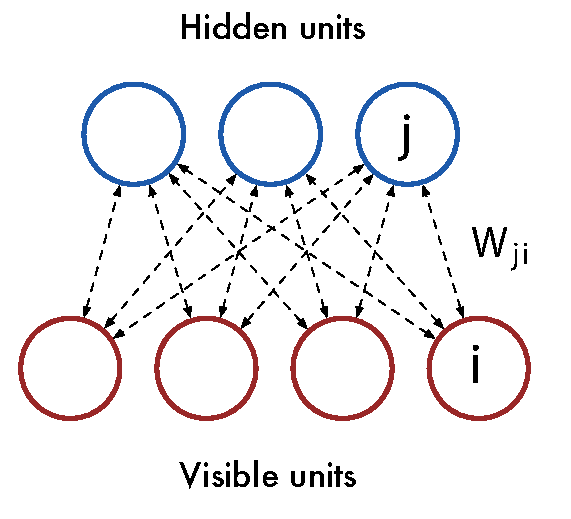
\includegraphics[scale=0.6]{RBM.pdf}
		\caption{The \textit{Restricted Boltzmann Machine} (RBM) is defined by a set of visible ($v_{i}$) and hidden ($h_{j}$) units.  Symmetric weights ($W_{ij}$) connect a hidden unit to a visible unit which altogether define an energy function $E_{W}(v,h)$. Training an \textit{RBM} consists in modifying the weights $W$ to lower the energy function around the points observed in the training set.}
		\label{fig:RBM}
	\end{figure}
	
	\subsection{Conditional RBM}
	The conditional \textit{RBM} (\textit{cRBM}) model \cite{taylor2009factored} is an extension of the \textit{RBM} in which dynamic biases are added to the biases of the visible ($\bm{a}$) and hidden ($\bm{b}$) units (see \prettyref{fig:cRBM_orchestration}). These dynamic biases linearly depend on a set of $K$ context units denoted $\bm{x} = (x_{1},...,x_{K})$, and the sum of the static and dynamic biases is equal to
	\begin{align*}
	\hat{a}_{i}(t) &= a_{i} + \sum_{k}A_{ki}x_{k}(t)\\
	\hat{b}_{j}(t) &= b_{j} + \sum_{k}B_{kj}x_{k}(t)
	\end{align*}
	In the case of time series, if the visible units represent a frame at time $t$, these context units can be used to model the influence of the recent past frames $\left[ t-N, t-1 \right]$ on the current frame ($N$ defining the \textit{temporal order}).
	Thus, the energy function of the \textit{cRBM} is given by
	\begin{equation}
	\begin{split}
	\label{eq:energy_cRBM}
	E(\bm{v}(t),\bm{h}(t)|\bm{x}(t)) =  - \sum_{i} \hat{a}_{i}(t)v_{i}(t) - \\ \sum_{ij}W_{ij}v_{i}(t)h_{j}(t) - \sum_{j} \hat{b}_{j}(t)h_{j}(t)
	\end{split}
	\end{equation}
	
	This model can be trained using CD, since the marginal probabilities of visible and hidden units are the same as the \textit{RBM} (simply replacing the static biases by dynamics ones).
	Hence, the update rules are unchanged for $\bm{W}$, $\bm{a}$ and $\bm{b}$, and
	\begin{align}
	\Delta A_{ik} 	&=<v_{i}x_{k} >_{data} - <v_{i}x_{k} >_{model}\\
	\Delta B_{jk} 	&= <h_{j}x_{k} >_{data} - <h_{j}x_{k} >_{model}
	\end{align}
	
	\begin{figure}[ht]
		\centering
		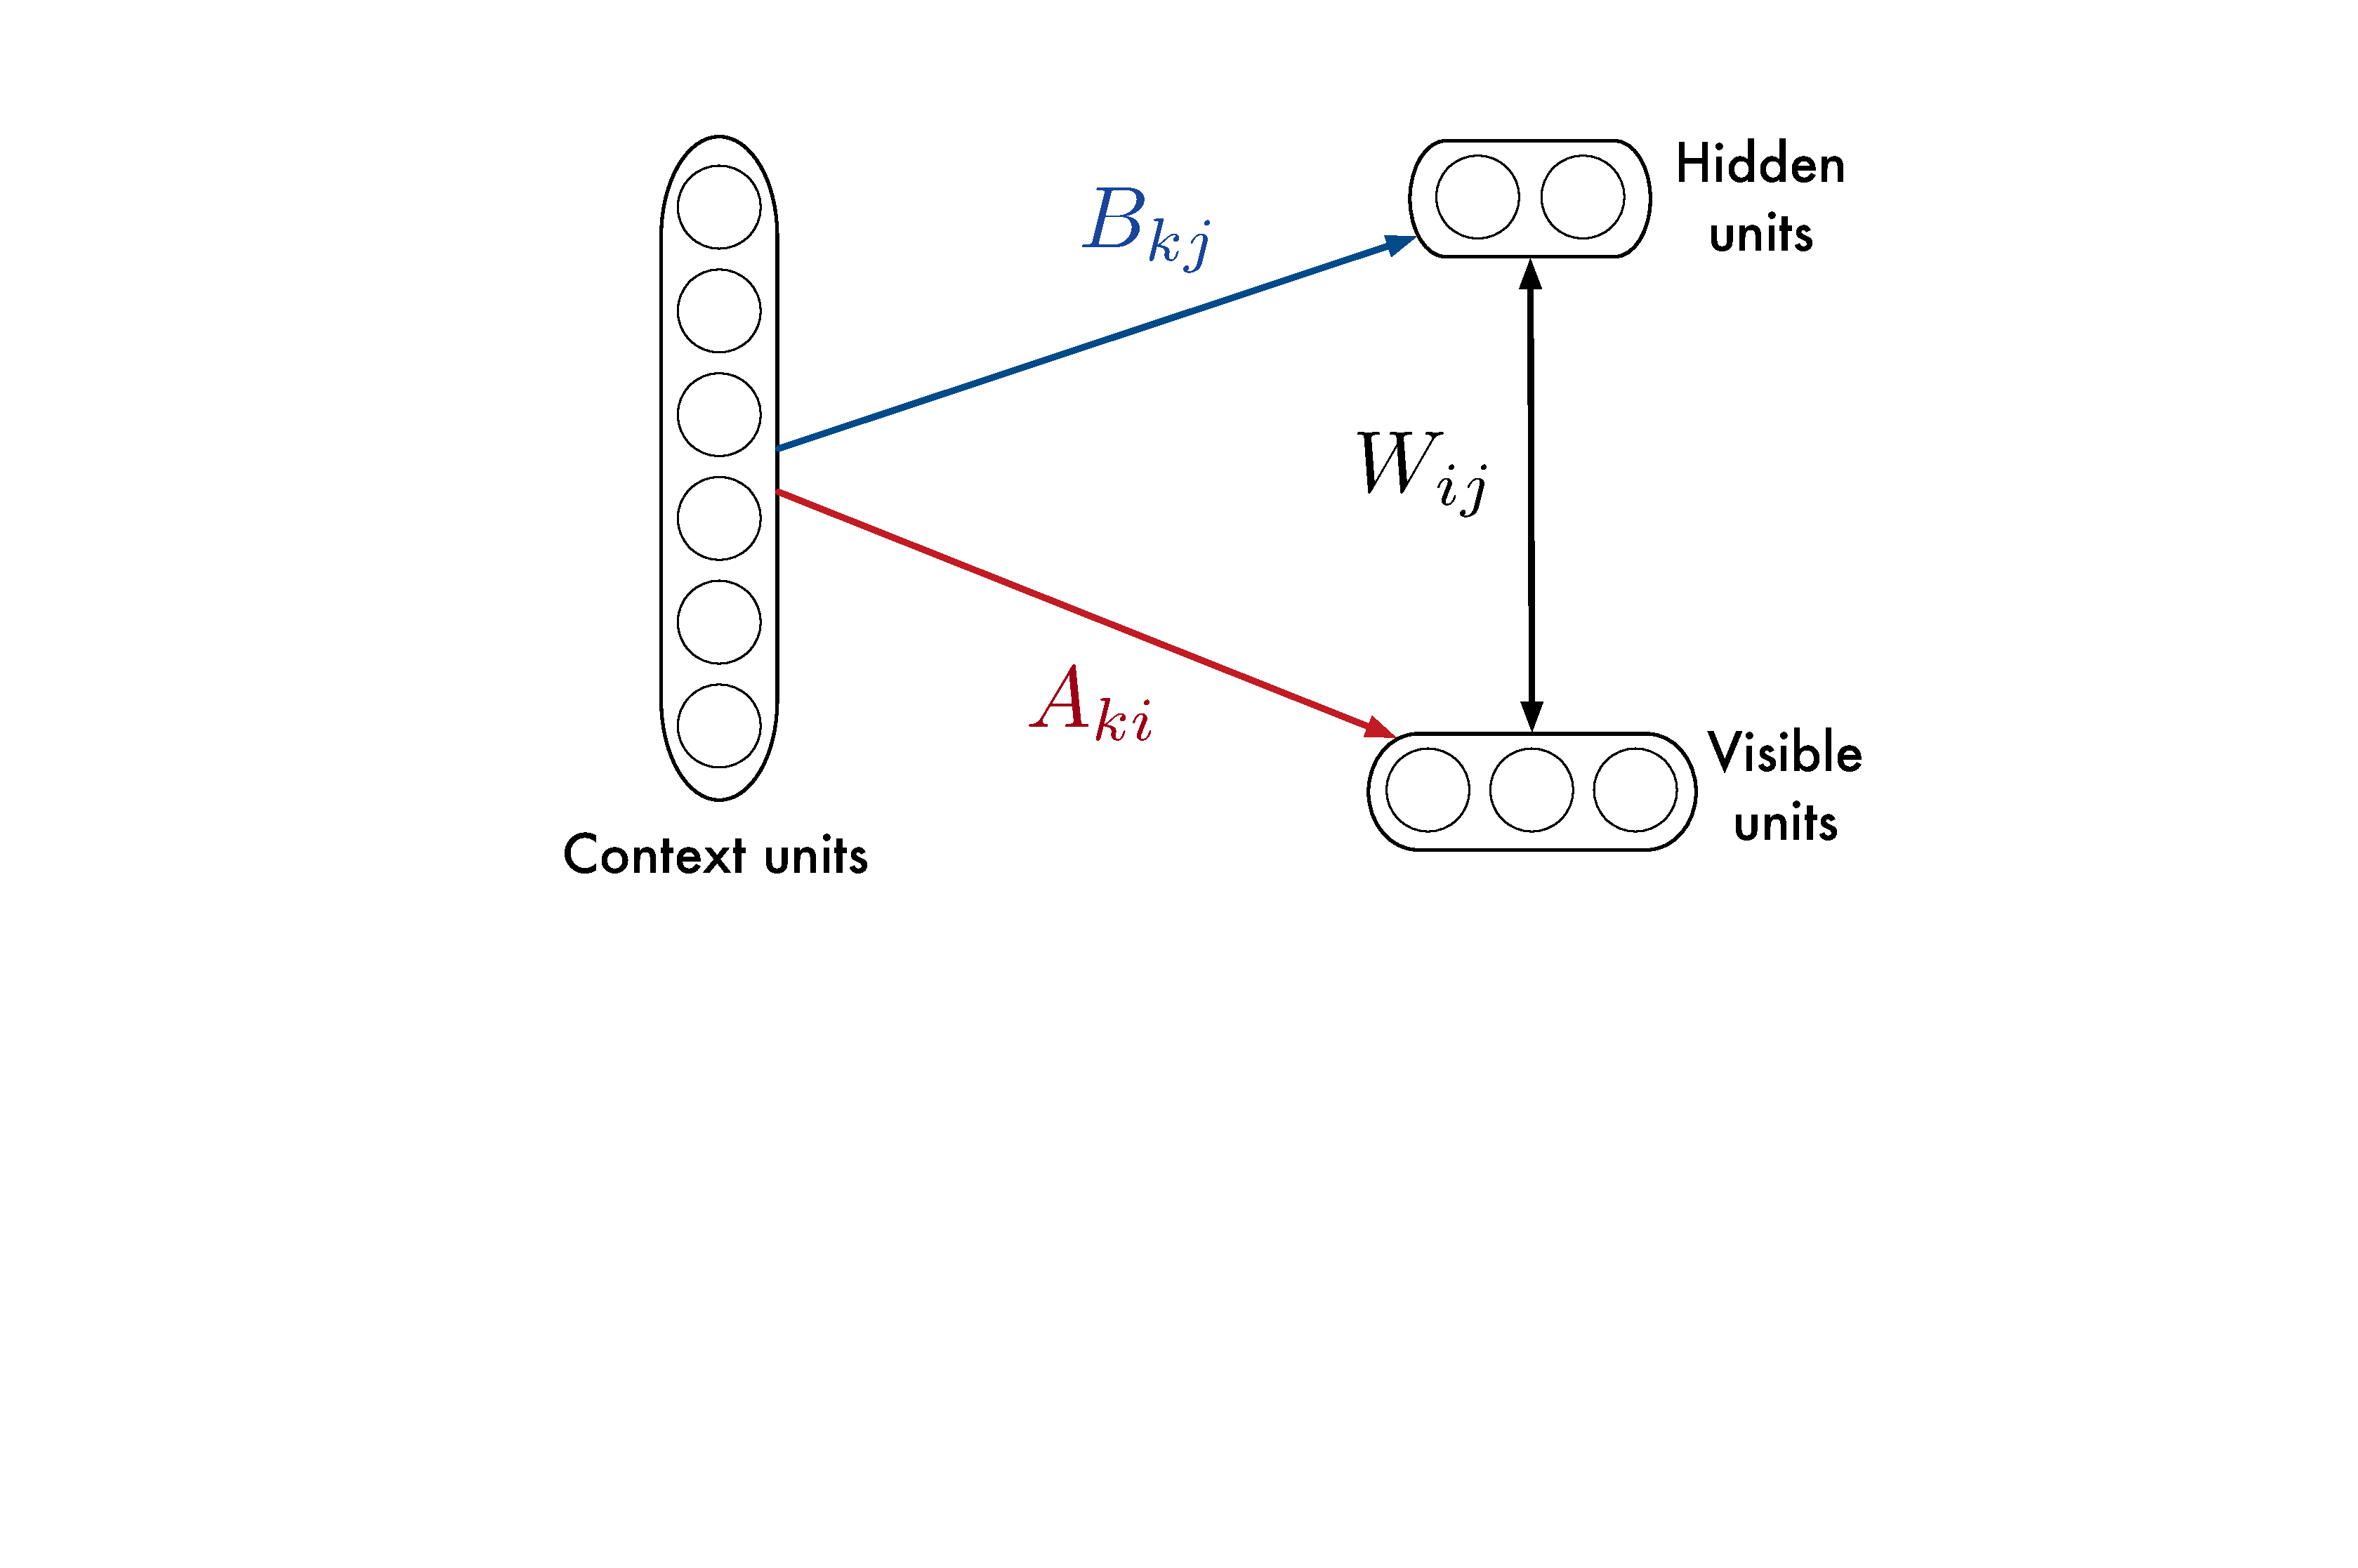
\includegraphics[scale=0.26]{cRBM_orchestration.pdf}
		\caption{\textit{The conditional RBM} (\textit{cRBM}) adds a layer of context units to the standard RBM architectures. Those context units linearly modify the biases of both the visible and hidden units through the dynamics terms.}
		\label{fig:cRBM_orchestration}
	\end{figure}
	
	\subsection{Factored Gated cRBM}
	The Factored Gated cRBM (\textit{FGcRBM}) model  \cite{taylor2009factored} proposes to extend the cRBM model by adding a layer of feature units $\bm{z}$ which modulates the weights of the conditional architecture in a multiplicative way (see \prettyref{fig:FGcRBM}). Hence, the parameters of the model become $\bm{\theta} = \left\lbrace \bm{W} , \bm{A} , \bm{B} , \bm{a} , \bm{b} \right\rbrace$, where $\bm{W} = (W)_{ijl}$, $\bm{A}=(A)_{ikl}$ and $\bm{B}=(B)_{jkl}$ are three-dimensional tensors.
	
	This multiplicative influence can be interpreted as a modification of the energy function of the model depending on a for of style features. For a fixed configuration of feature units, a new energy function is defined by the \textit{cRBM} ($\bm{v}$, $\bm{h}$, and $\bm{x}$). The number of parameters grows cubically with the number of units. To reduce the computation load, the three dimensional tensors can be factorized into a product of three matrices by including factor units indexed by $f$ such that $W_{ijl} = W_{if} . W_{jf} . W_{lf}$.
	The energy function of the \textit{FGcRBM} is then given by
	\begin{equation}
	\begin{split}
	E(\bm{v}(t),\bm{h}(t)|\bm{x}(t),\bm{z}(t)) = - \sum_{i} \hat{a}_{i}(t)v_{i}(t) - \\ \sum_{j} \hat{b}_{j}(t)h_{j}(t)
	-\sum_{f}\sum_{ijl} W_{if}^{v} W_{jf}^{h} W_{lf}^{z} v_{i}(t) h_{j}(t) z_{l}(t) 
	\end{split}
	\end{equation}
	where the dynamic biases of the visible and hidden units are defined by
	\begin{equation}
	\hat{a}_{i}(t) = a_{i} + \sum_{m} \sum_{kl}A_{im}^{v}A_{km}^{x}A_{lm}^{z}x_{k}(t)z_{l}(t)
	\end{equation}
	\begin{equation}
	\hat{b}_{j}(t) = b_{j} + \sum_{n} \sum_{kl}B_{jn}^{h}B_{kn}^{x}B_{ln}^{z}x_{k}(t)z_{l}(t)
	\end{equation}
	
	\begin{figure}[ht]
		\centering
		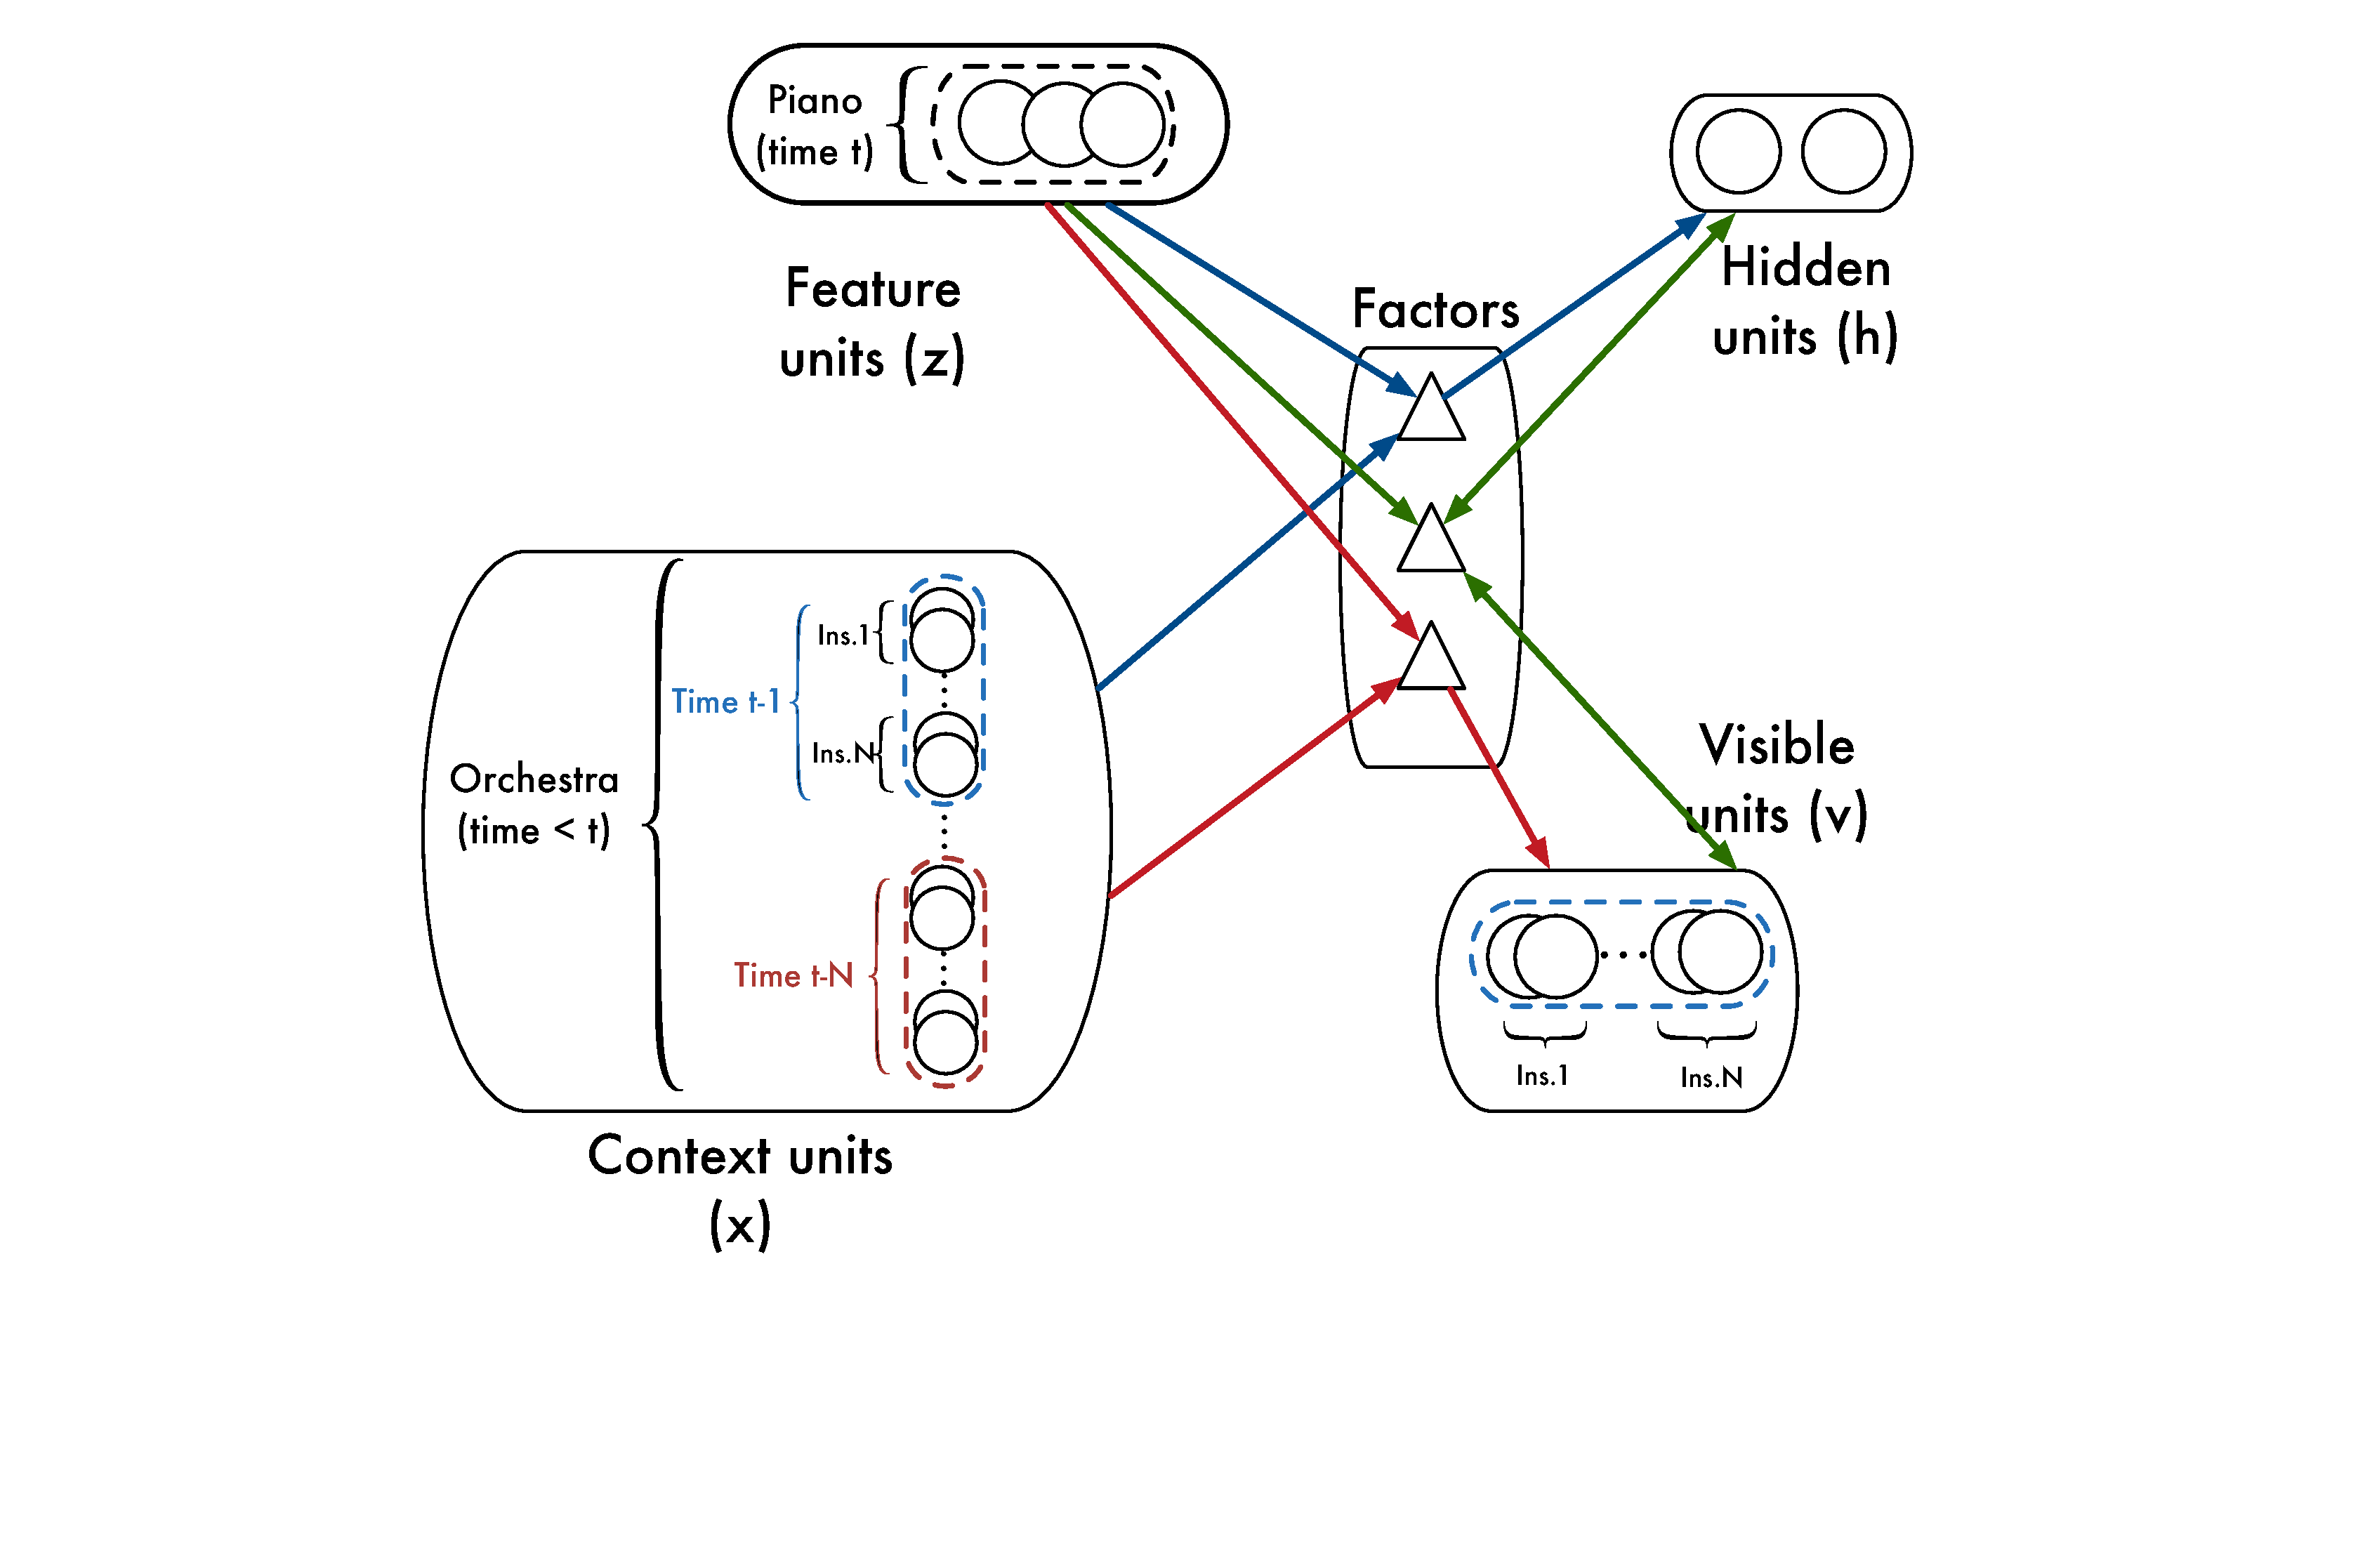
\includegraphics[scale=0.20]{FGcRBM_orchestration.pdf}
		\caption{\textit{FGcRBM} model. The features units ($\bm{z}$) modify the energy landscape of the model through a multiplicative influence over the weights $\bm{A}$, $\bm{B}$ and $\bm{W}$. Here, the role of each unit in the context of orchestration is indicated.}
		\label{fig:FGcRBM}
	\end{figure}
	
	\subsection{Sampling from the models}
	% Role des unités conditionelles et tout le tralala dans les modèles
	Using gradient descent during the learning phase brings no guarantee over the quality of the approximation between the model distribution and the data distribution.
	However, \textit{CD} guarantees that the Kullback-Leibler divergence between the model and data distribution is reduced after each iteration\cite{hinton2002training}, and an acceptable approximation should be found after large number of \textit{CD} steps.
	Therefore, by sampling from the model distribution, we are able to generate novel data \textit{similar} to the one observed in the training dataset but yet unseen. In practice, sampling from the conditional models is performed by computing the marginal distribution of the visible units knowing the context $p(v|x) = \sum_{h} p(v,h|x)$, and then sampling from a Bernoulli distribution of parameter $p(v|x)$.
	Unfortunately, this marginal distribution remains computationally intractable in the introduced models because of the partition function. However, samples from an approximate distribution can be reached through alternate Gibbs sampling. After randomly setting the visible units (for each index $i$, $\bm{v}_{i} \sim \mathcal{U}(0,1)$), K Gibbs sampling steps are performed to obtain a visible sample. The objective of these K steps is to reach the equilibrium distribution of the model. Even though a theoretically  infinite number of steps is necessary, 20 to 100 steps are typically sufficient.
	Note that, in practice, a threshold is applied on the activation of the visible units before the last sampling step in the \textit{Gibbs chain} so that unlikely activations are set to zero.
	
	\begin{figure}
		\centering
		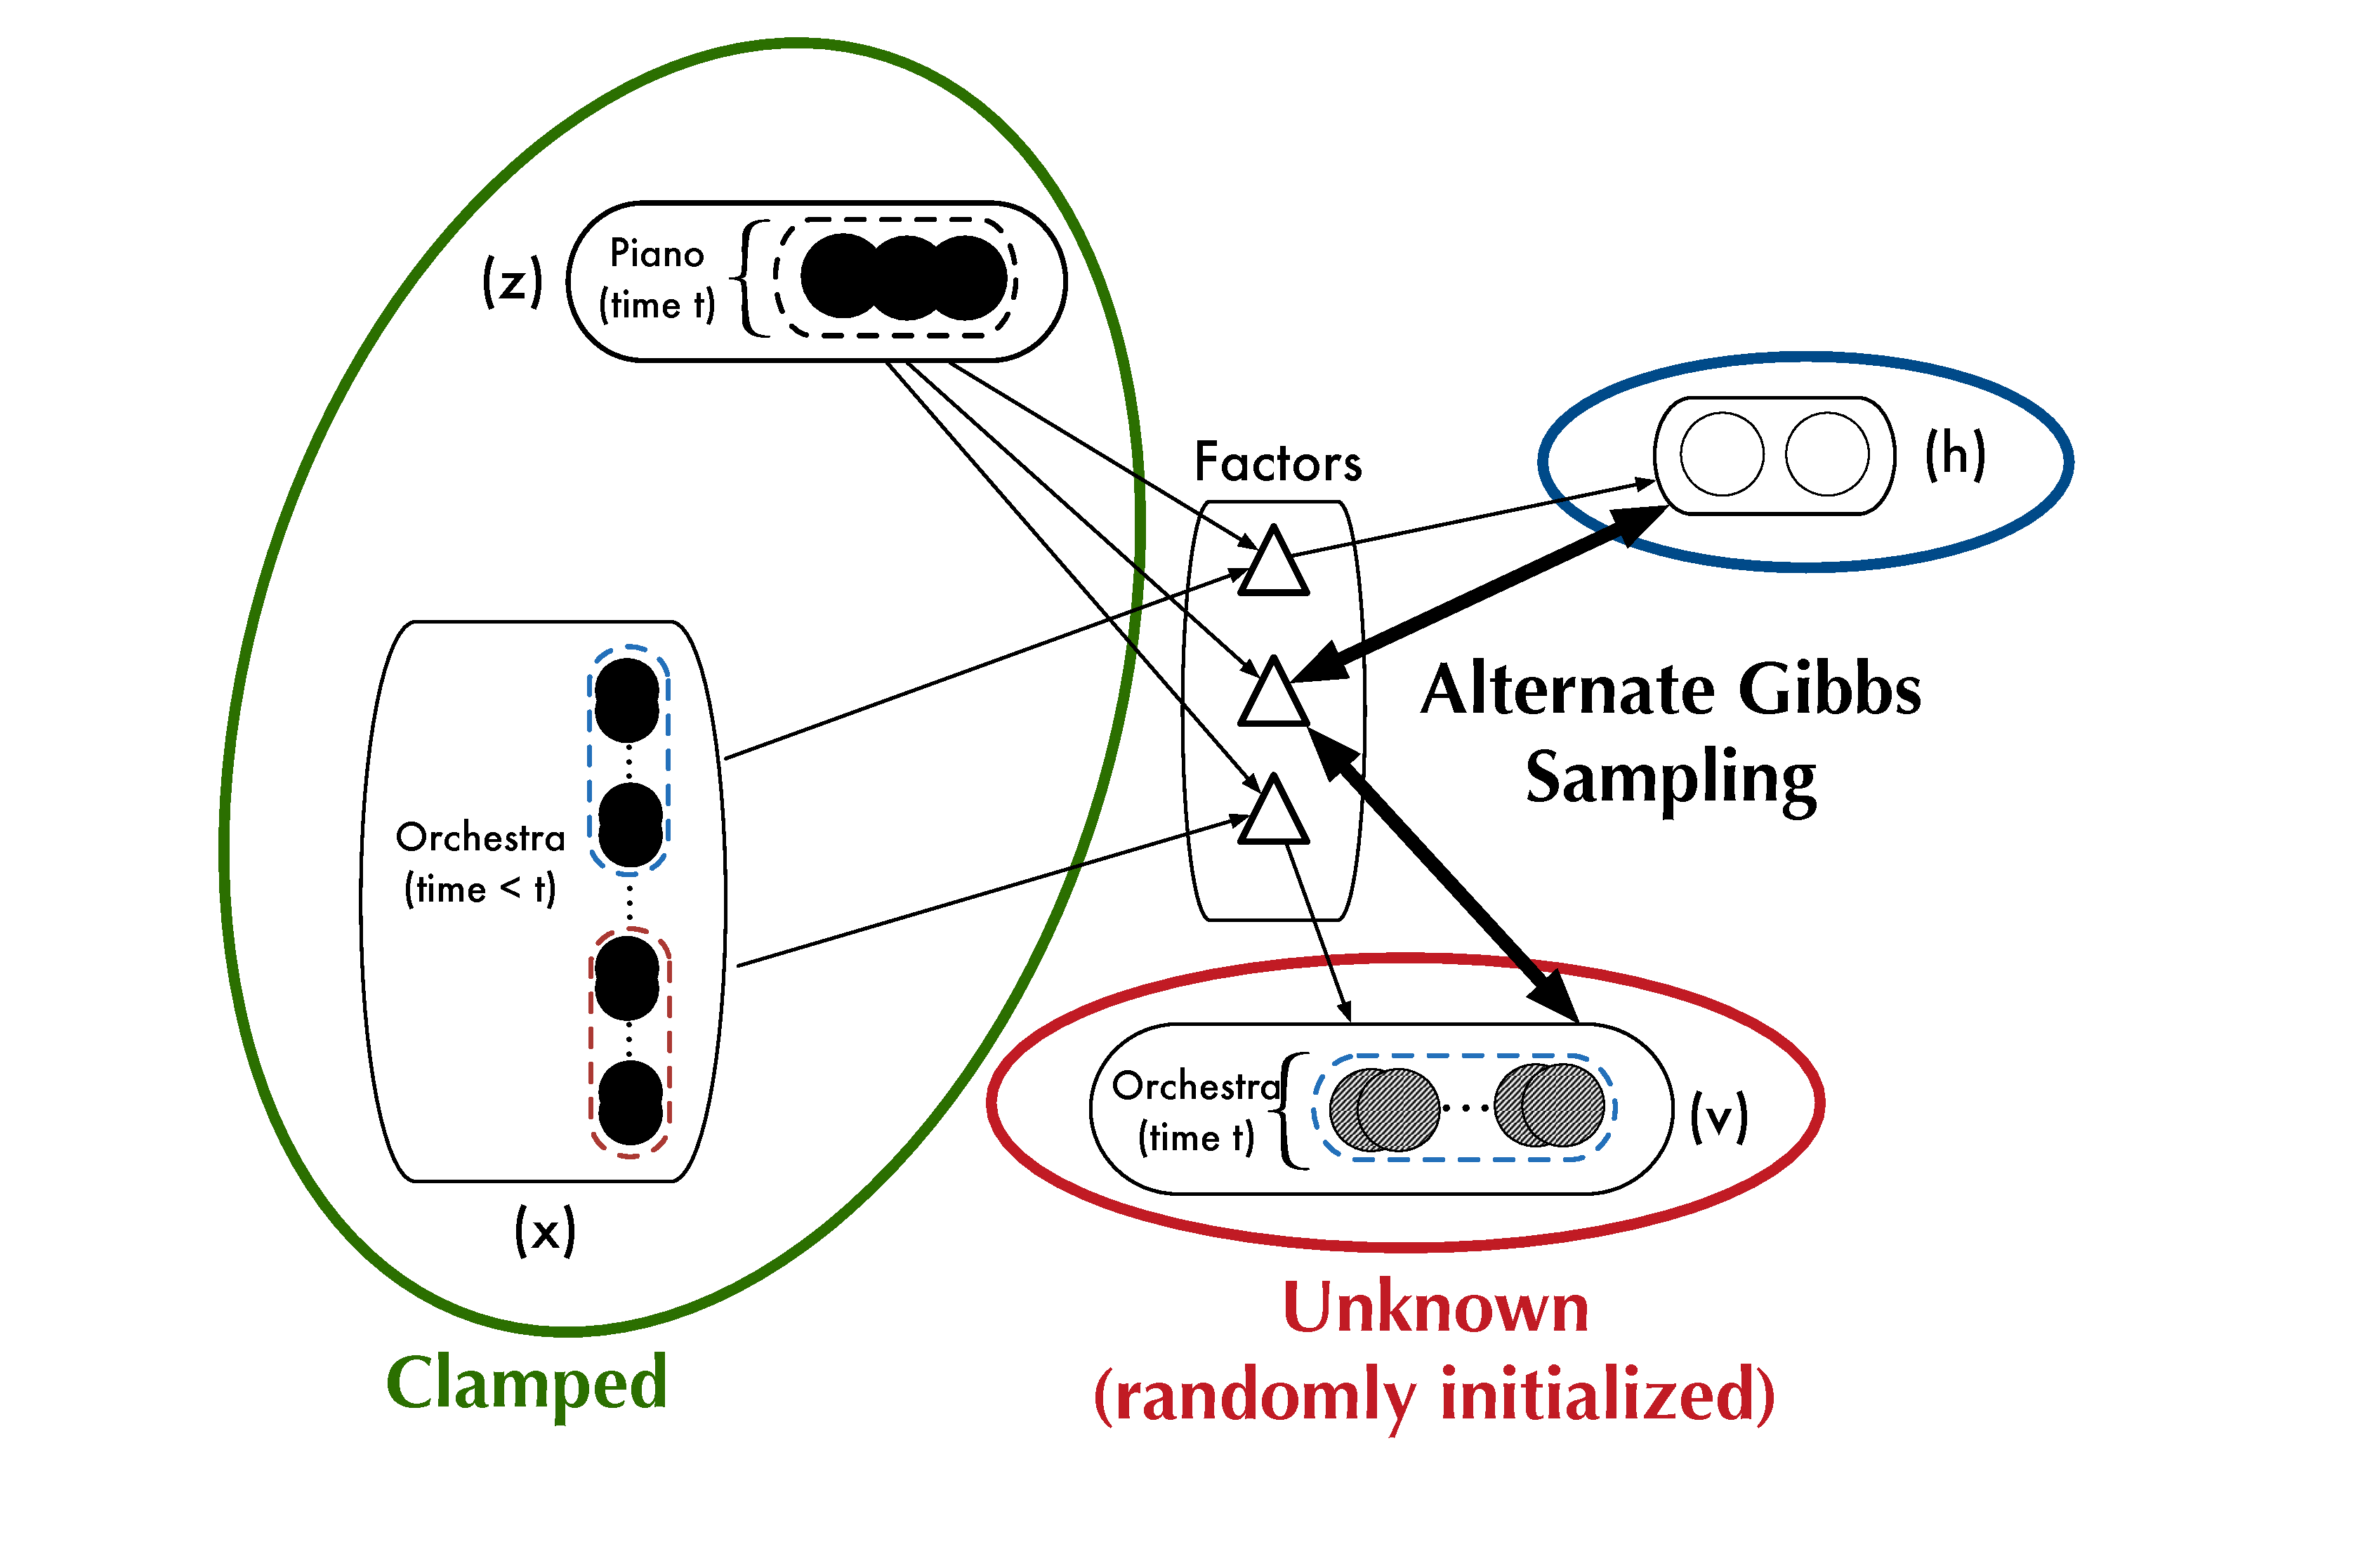
\includegraphics[scale=0.14]{FGcRBM_sampling.pdf}
		\caption{\textit{Sampling in a FGcRBM}. Context and feature units are respectively clamped to the last ($t-1$ to $t-N$) orchestral frames and the current ($t$) piano frame. Visible units are randomly initialized. Then, several Gibbs sampling step are performed until reaching the equilibrium distribution of the model.}
		\label{fig:FGcRBM_sampling}
	\end{figure}
	
	\section{Projective orchestration}
	In this section, we introduce and formalize the automatic projective orchestration task presented in \prettyref{fig:orch}. In particular, we detail the database and data representation used, evaluation framework, and discuss the results obtained by different models.
	
	\subsection{Database}
	We use a database of piano scores and their orchestration by famous composers. The database consists of 76 excerpts of orchestral pieces, and fourteen different instruments were present in the database. This database has been collected by orchestration teachers and are the transcription of famous composers orchestration in the \textit{MusicXML} format.
	
	\subsection{Data representation}
	In order to process the scores, we import them as matrices called \textit{piano-roll}, a data representation traditionally used to model polyphonic music of a single instrument (see \prettyref{fig:piano-roll}). 
	Its extension to represent an orchestra is straightforwardly obtained by the concatenation of the \textit{piano-rolls} of each instrument along the pitch dimension.
	
	The rhythmic quantization is defined as the number of time frame in the \textit{piano-roll} per quarter note. When constructing the piano-rolls, we used a rhythmic quantization of 4.
	
	In order to reduce the number of units, we systematically remove, for each instrument, any pitch which is never played in the training database. Hence, the dimension of the orchestral vector decreased from 2432 to 456 and the piano vector dimension from 128 to 88.
	Also, we follow the classic orchestral simplifications used when writing orchestral scores by grouping together all the instruments of the same section. For instance, the \textit{violin} section, which might be composed by several instrumentalists, is written as a single part.
	Finally, the velocity information is discarded, since we use binary units which solely indicate if a note is on or off.
	
	\begin{figure}[ht]
		\centering
		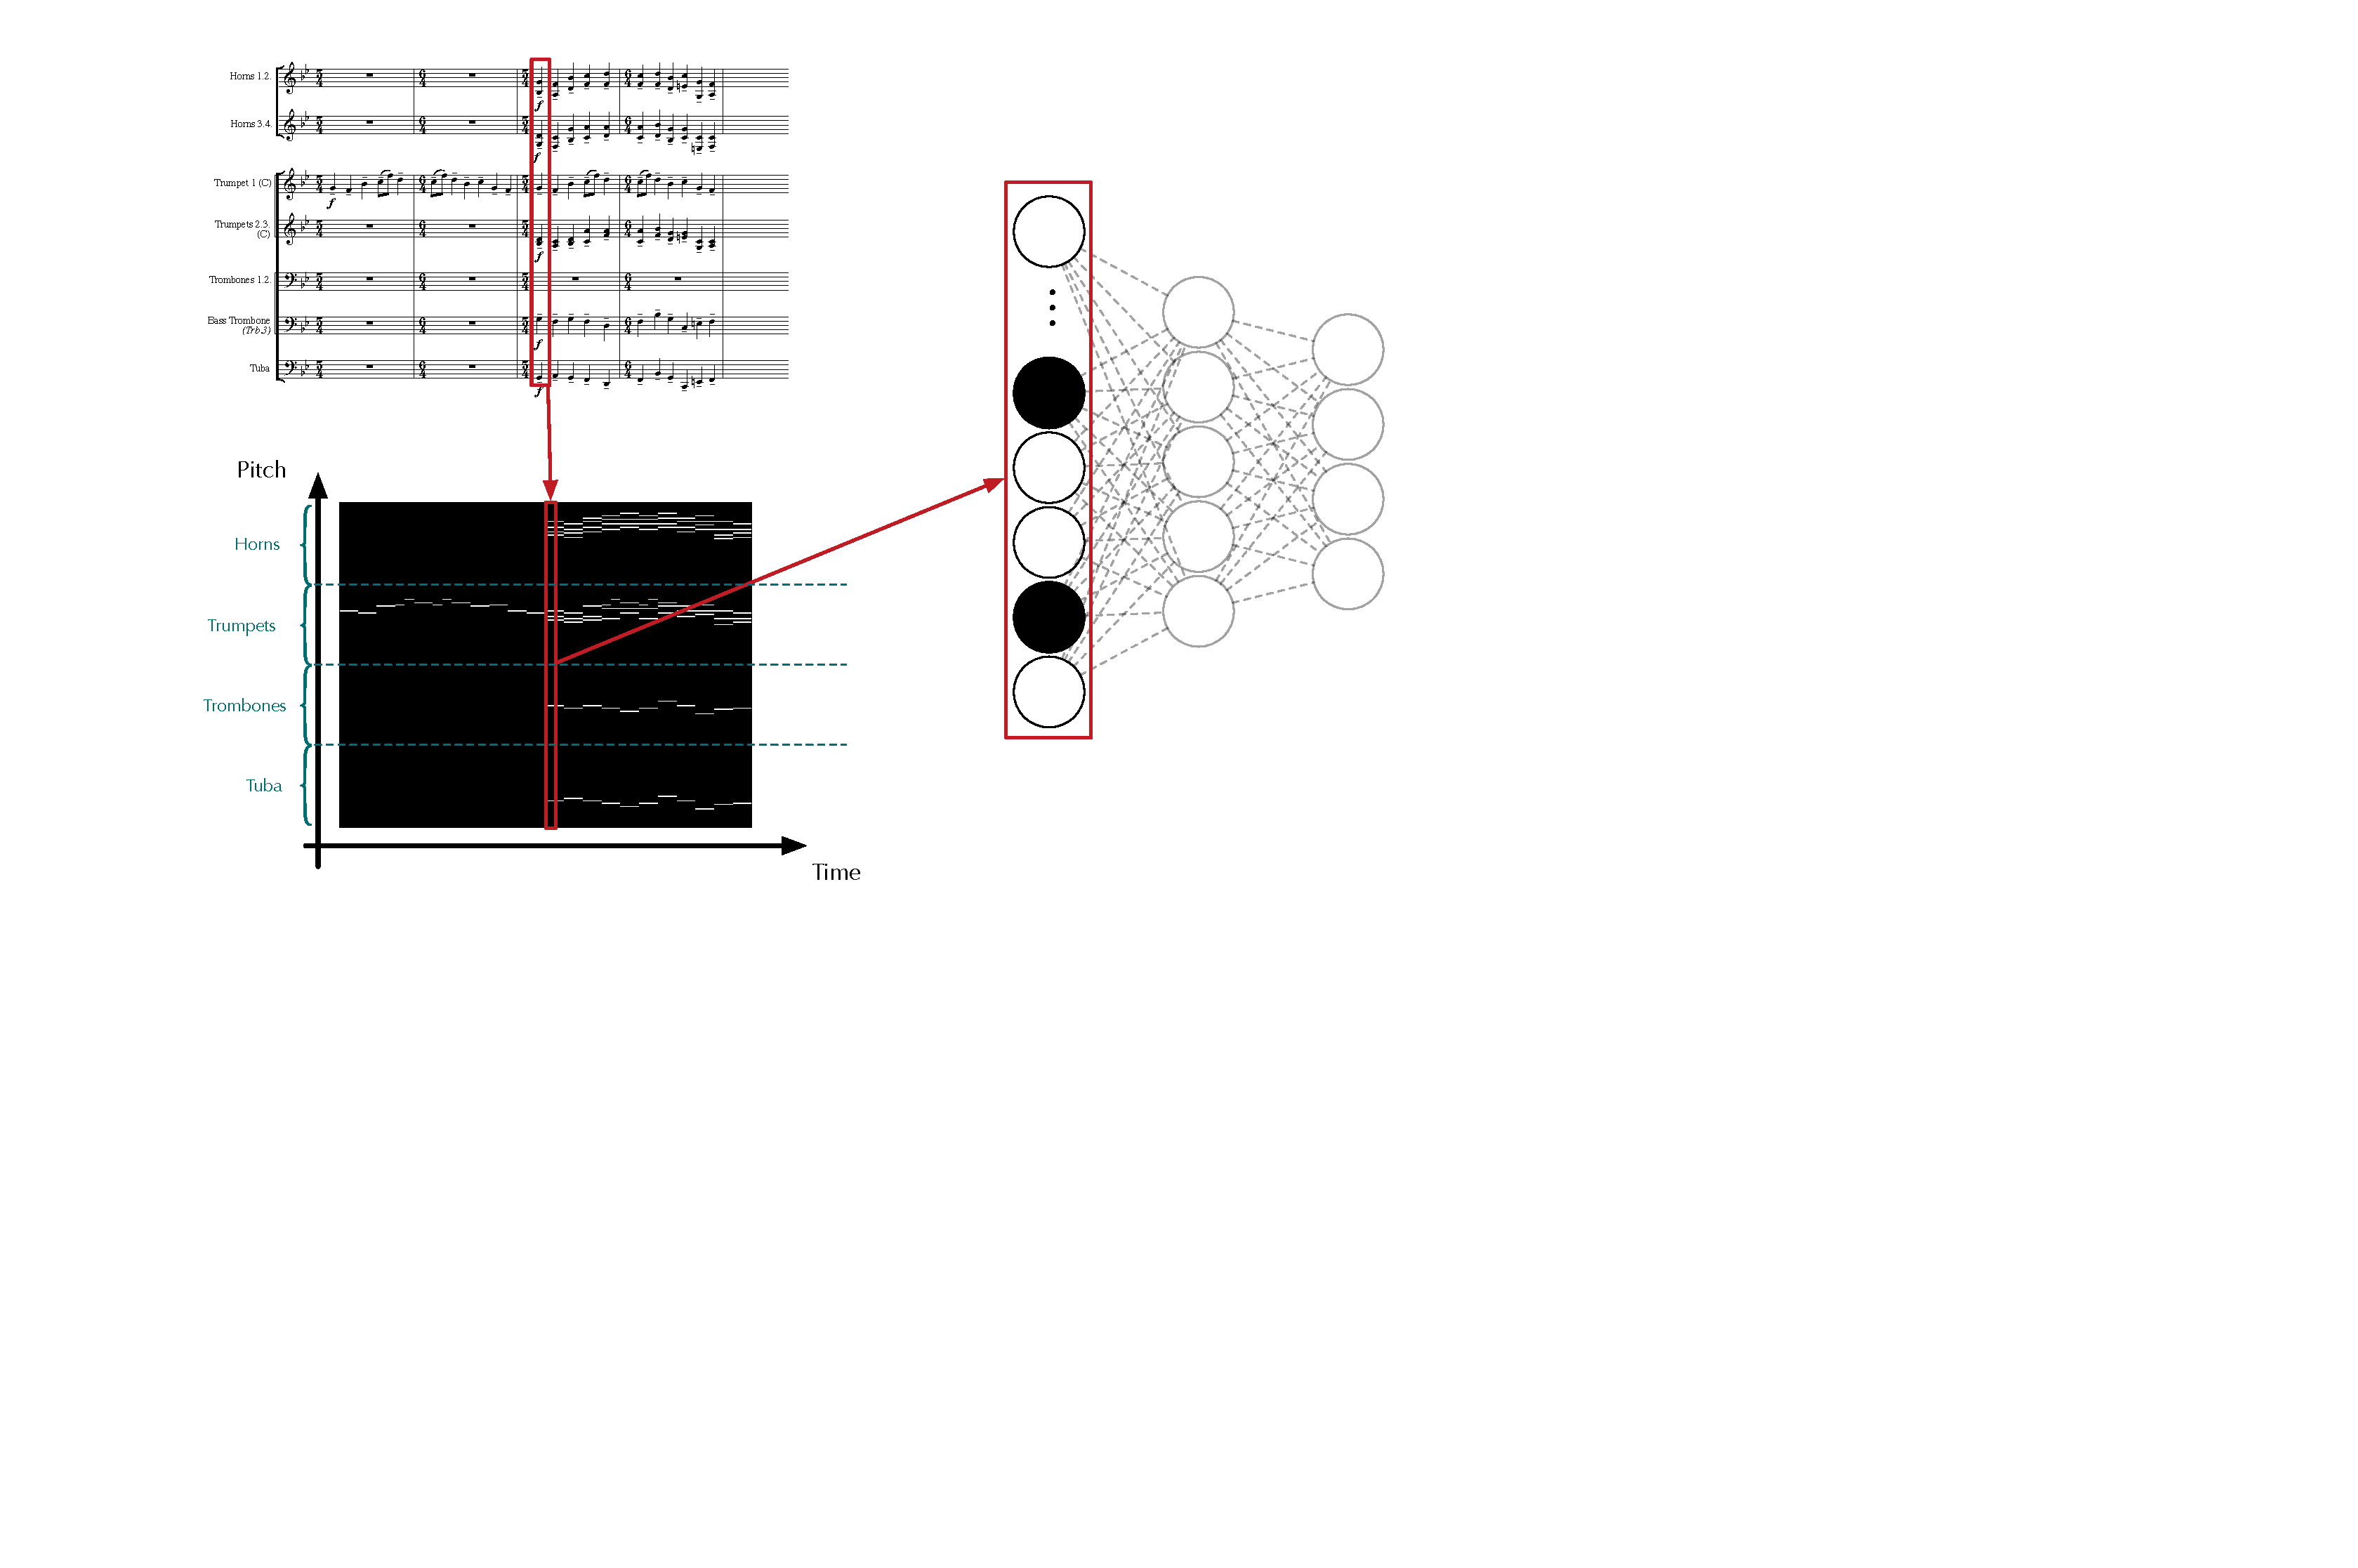
\includegraphics[scale=0.35]{data_representation.pdf}
		\caption{From the score of an orchestral piece, a convenient representation for computer processing named \textit{piano-roll} is extracted. A piano-roll $pr$ is a matrix whose rows represent pitches and columns represent a time frame depending on the discretization of time. A pitch $p$ at time $t$ played with an intensity $i$ is represented by $pr(p,t) = i$, $0$ being a note off. This definition is extended to an orchestra by simply concatenating the \textit{piano-rolls} of every instruments along the pitch dimension.
			Finally, each time frame in the piano-roll matrix will be modelled by the visible units of the \textit{RBM}, in order to learn the probability distribution of the orchestral process.}
		\label{fig:piano-roll}
	\end{figure}
	
	\subsection{Model definition}
	For each orchestral piece, we define $Orch(t)$ and $Piano(t)$ as the sequence of column vectors from the \textit{piano-roll} of the orchestra and piano part respectively, with $t \in \left[ 1,N_{T} \right]$ where $N_{T}$ is the length of the piece.
	
	At each time index $t$, the visible units of the \textit{cRBM} will model the current orchestral vector $Orch(t)$ that we want to generate. Conditional units are used to add the influence of the past orchestral vectors $Orch(t-1) , ... , Orch(t-N)$ and the influence of the current piano frame $Piano(t)$ over the visible units. Hence, in the \textit{cRBM} model, the context units at time $t$ are defined by the concatenation of the past orchestral frames and current piano frame
	\begin{equation}
	\bm{x}(t) = \left[ \text{Piano}(t) , \text{Orch}(t-1) , ... , \text{Orch}(t-N)\right]
	\end{equation}
	
	The \textit{FGcRBM} model allows to separate the influence of the current piano frame and the past orchestral frames. Hence, the current piano frame defines the feature units
	\begin{equation}
	\bm{z}(t) = \text{Piano}(t)
	\end{equation}
	while the concatenation of the past orchestral frames defines the context units
	\begin{equation}
	\bm{x}(t) = \left[ \text{Orch}(t-1)^{T} , ... , \text{Orch}(t-N)^{T} \right]
	\end{equation}
	
	\subsection{Evaluation framework}
	We introduce an \textit{event-level orchestral inference} task to evaluate our models. To our best knowledge, this is the first attempt to define a quantitative evaluation framework for automatic projective orchestration.
	
	In order to evaluate the models, the data used to train and those used to assess the performances must be different \cite{bishop2006pattern}. Hence, the dataset is usually split between a train and test set.
	Given the complexity of the distribution we want to model and the extremely narrow size of the database, we rely on a Leave-One-Out (\textit{LOO}) evaluation where 75 scores are used to train the model and one is kept for testing. This choice is motivated by the will to obtain the best generative model possible.
	
	Predictive symbolic music tasks are usually evaluated through a \textit{frame-level} accuracy measure where each time frame of the piano-roll is considered as a separate data example \cite{DBLP:journals/corr/YaoCVDD15,boulanger2012modeling,lavrenko2003polyphonic}.
	We propose to work in an \textit{event-level} framework, where data examples are only those for which an event occurs. An event is defined as a time $t_{e}$ where $\text{Orch}(t_{e}) \neq \text{Orch}(t_{e} - 1)$. The reason why we do not rely on a \textit{frame-level} evaluation is that a model which simply repeats the previous frame gradually becomes the best model as the quantization gets finer. Moreover, in the projective orchestration framework, rhythmic patterns are already established by the known piano score and, thus, does not have to be learned by the model.
	
	% Nombre de batch
	Finally, to speed-up the convergence of the gradient descent, mini-batches are used to train the model \cite{bishop2006pattern}. Following these procedures, 89 mini-batches of 100 event-level points were obtained for training.
	
	\subsection{Measure}
	An objective criterion of the performances of the models is necessary to provide an evaluation. 
	The best way for evaluating generative models is to compute the likelihood of the test set (see equation \prettyref{eq:likelihood}). However, we have seen that this quantity is intractable in all \textit{RBM}, \textit{cRBM} and \textit{FGcRBM} models. 
	An alternative criterion commonly used in the music generation field is the accuracy measure \cite{DBLP:journals/corr/YaoCVDD15,boulanger2012modeling,lavrenko2003polyphonic}. For each \textit{event} $t_{e}$ (see previous section), the visible units of the model are sampled with its context (and features for the FGcRBM) units set to $Orch(t_{e}-1),... Orch(t_{e}-N)$ and $Piano(t_{e})$ from the test dataset. This sampled prediction $\text{Pred}(t_{e})$ is then compared to the ground-truth vector $\text{Orch}(t_{e})$ from the test dataset via the accuracy measure
	\begin{equation}
	\text{Accuracy}  = \frac{TP(t)}{TP(t) + FP(t) + FN(t)}
	\label{eq:accuracy}
	\end{equation}
	where $TP(t)$ (true positives) is the number of notes correctly predicted (note played in the prediction and ground-truth). $FP(t)$ (false positive) is the number of notes predicted which are not in the original sequence (note played in the prediction, but not in ground-truth). $FN(t)$ (false negative) is the number on unreported notes (note absent in prediction, but played in ground-truth). 
	Instead of binary values, activation probabilities are used for the predicted samples in order to avoid sampling noise.
	
	\subsection{Results}
	Four models are evaluated on the orchestral inference task. The first model is a random generation of the orchestral frames from a Bernoulli distribution of parameter $0.5$. The second model predicts an orchestral frame at time $t$ by repeating the frame at time $t-1$. Those two naive models constitute a first baseline against which we compare the cRBM and FGcRBM models.
	
	The results are summed up in \prettyref{tab:result_event_level}. As expected, the random model has poor results. The repeat model performs significantly better. Indeed, it is relatively common that a note is sustained between two successive events. The cRBM largely outperforms those two models. However, the FGcRBM model has a lower score than the repeat model. We observed that the activation function of the visible units during the generative step was extremely noisy, which suggests that the training procedure mostly failed. We believe that this is due to the number of parameter,  and especially the dimension of the feature units. Indeed, in \cite{taylor2009factored}, only ten different configuration of the feature units were possible. When training on an orchestral database,  each different piano frame define a different configuration.
	
	\begin{table}[h]
		\centering
		\begin{tabular}{c c}
			\hline
			Model & Orchestral Event-level (\%)\\
			\hline
			Random & 0.5\\ 
			Repeat & 12.6\\
			\hline \hline
			cRBM & 23.2\\ 
			FGcRBM & 6.2\\ 
		\end{tabular}
		\caption{Event-level accuracy for the orchestral inference task. Even though the cRBM performances increase by a factor 3 between the cRBM and the random model, the inclusion of features units provides a leap in the accuracy by multiplying the performances by 4.}
		\label{tab:result_event_level}
	\end{table}
	
	\subsection{Discussion : evaluating a generative model ?}
	It is important to state that we do not consider this predictive measure as as reliable measure of the creative performance of a model. Indeed, predicting and creating are two fairly different things. 
	Hence, the predictive evaluation framework we have built does not assess the generative ability of a model, but is rather used as a selection criterion among different models.
	
	%As pointed out in \cite{boulanger2012modeling}, a better evaluation measure would be the likelihood of a sequences from a test dataset. Unfortunately, these quantities are computationally intractable in the introduced models. However, recent works estimator of the partition function 
	
	\section{Live Orchestral Piano (LOP)}
	We introduce in this section the \emph{Live Orchestral Piano} (LOP)
	application, which is the first software able to provide a way to
	compose music with a full classical orchestra in real-time by simply
	playing on a MIDI piano. The goal of this framework is to rely on
	the knowledge learned by the model introduced in the previous sections
	in order to perform the projection from a piano melody to the orchestra.
	
	\subsection{Workflow}
	The software is implemented on a client/server paradigm. This choice
	allows to separate the orchestral computation part from the interface
	and sound rendering engine. That way, multiple interfaces can easily
	be implemented. It should also be noted that separating the computing
	and rendering on different computers, can allow to use high-quality
	and CPU-intensive orchestral rendering plugins. This can allow a more
	realistic orchestral rendering with heavy amounts of computation performed
	while ensuring the real-time constraint on the overall system (preventing
	degradation of the computing part). The complete implementation workflow
	is presented in Figure~\ref{fig:Live-orchestral-piano}.
	
	\begin{figure*}
		\begin{centering}
			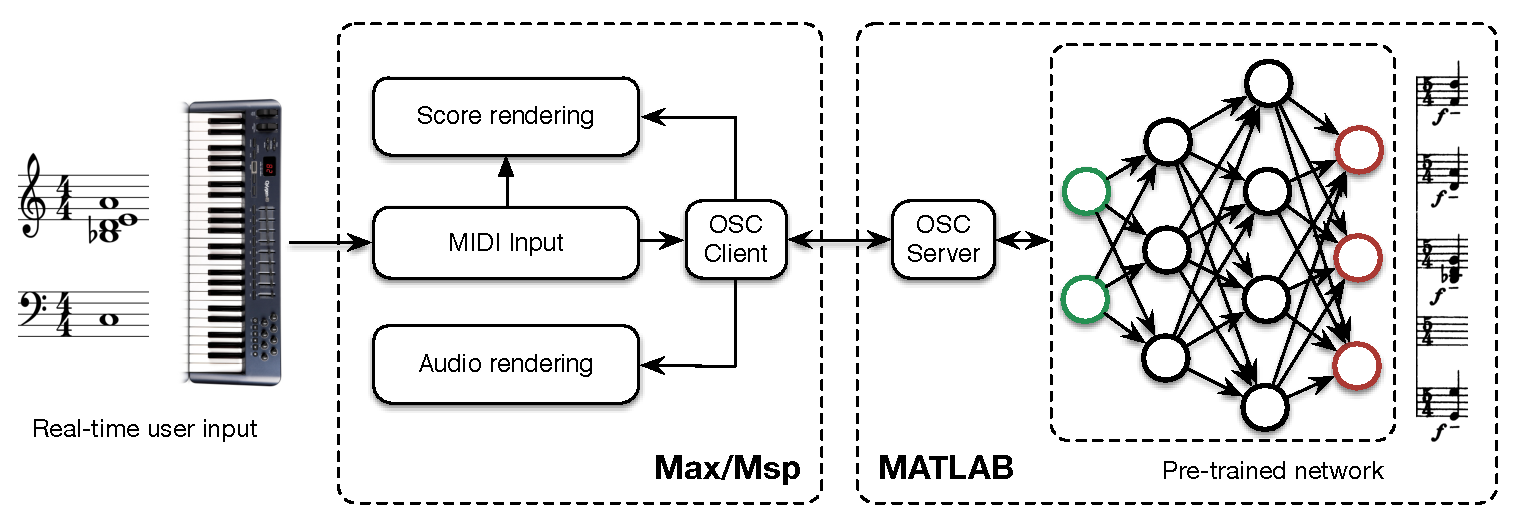
\includegraphics[scale=0.55]{workflow.pdf}
			\par\end{centering}
		
		\caption{\label{fig:Live-orchestral-piano}Live orchestral piano (L.O.P) implementation
			workflow. The user inputs a melody which is transcribed into a score
			and send via OSC from the Max/Msp client. Then, the MATLAB server
			uses this vector of notes and process it following the aforementioned
			techniques in order to obtain the orchestration. This information
			is then sent back to Max/Msp which performs the real-time audio rendering }
	\end{figure*}
	
	As we can see, the user can input a melody (single notes or chords)
	through a MIDI keyboard, which is retrieved inside the Max/Msp interface.
	The interface transmits this symbolic information (as a variable-length
	vector of active notes) via OSC to the MATLAB server. The interface
	performs a real-time transcription of the piano score to the screen
	in parallel. The server uses this vector of events to produce an 88
	vector of binary input note activations (as defined in the sub-section \textit{Data representation}).
	This vector is then processed by using the orchestration algorithms
	presented in sub-section \textit{Model definition} in order to obtain a projection
	of a specific symbolic piano melody to the full orchestra (an operation
	defined as \emph{projective orchestration}). The resulting orchestration
	is then sent back to the client interface which performs both the
	real-time audio rendering and score transcription. 
	
	\subsection{Interface}
	The interface has been developed in Max/Msp, to facilitate both the
	score and audio rendering aspects in a real-time environment. The
	score rendering is handled by the \emph{Bach} library environment. 
	This interface provides a way to easily switch between different orchestration models, while controling other
	meta-parameters of the sampling. For instance the \emph{cutoff probability
	}gives a direct access to the density of the generated orchestration
	(in terms of number of played instruments). Indeed, a low cutoff probability
	implies that most activation of notes will be taken into account in
	the playback, while a high cutoff will produce more sparse orchestration.
	
	\section{Conclusion and future works}
	% Orchestral inf problem
	We have introduced a system for real-time projective orchestration of a midi piano input. In order to select the most adapted model, we have proposed an evaluation framework called orchestral inference which rely on an orchestral inference task. We have assessed the performance of the cRBM and FGcRBM, and observed the better performances of the cRBM model.
	
	% Interesting and highly benefit problem
	The general objective of building a generative model for time series is one of the most prominent topic for the machine learning field. Orchestral inference sets a slightly more specific framework where the generated time series is conditioned by an other observed time series (the piano score). Besides, being able to grasp the long range dependencies structuring music appears as a challenging and worthwhile task.
	
	% Increase DB
	The high dimensionality of the data and their sparsity are a major obstacle for learning algorithms.
	A first remark is that a larger database would be required to train any model sufficiently complex to properly represent the underlying distribution of a projective orchestration.
	It is important to build a reference database of piano scores and their orchestration by acknowledge composers, with all instrument name indicated and velocity for the notes. 
	% Velocities
	Indeed, we believe that taking the notes' velocity into consideration is crucial, since many orchestral effects are justified by intensity variations in the original piano scores. 
	% Find distrib representations
	Besides, the sparse representation of the data suggests that a more compact distributed representation might be found. Lowering the dimensionality of the data would greatly improve the efficiency of the learning procedure. For instance, methods close to the word-embedding techniques used in natural language processing might be useful \cite{kiros2015skip}.
	
	Finally, a better performance measure should be developed for the orchestral inference task. A solution could be to derive estimators for the likelihood of sequences under the proposed models. Recent work on methods such as Annealed Importance Sampling are promising.
	
	\section{Acknowledgements}
	This work has been supported by the \textit{NVIDIA GPU Grant} program.
	The authors would like to thank Denys Bouliane for kindly providing the orchestral database.
		
	
	\bibliographystyle{amsplain}
%	\bibliography{../Biblio/biblio}
	\bibliography{biblio}
	
\end{document}
